\documentclass[conference]{IEEEtran}
\IEEEoverridecommandlockouts
% The preceding line is only needed to identify funding in the first footnote. If that is unneeded, please comment it out.
\usepackage{cite}
\usepackage{amsmath,amssymb,amsfonts}
\usepackage{algorithmic}
\usepackage{graphicx}
\usepackage{textcomp}
\usepackage{xcolor}
\usepackage{listings}
\usepackage{pythonhighlight}
\usepackage{float}
\usepackage{hyperref}
\usepackage{verbatim}

\pagestyle{plain}

\def\BibTeX{{\rm B\kern-.05em{\sc i\kern-.025em b}\kern-.08em
    T\kern-.1667em\lower.7ex\hbox{E}\kern-.125emX}}
\begin{document}

% \hfuzz=500pt
\title{A Random Model of the Primes}
\author{\IEEEauthorblockN{1\textsuperscript{st} Yongyu Qiang}
\IEEEauthorblockA{\textit{Georgia Institute of Technology}}
\and
\IEEEauthorblockN{2\textsuperscript{nd} Aravinth Venkatesh Natarajan}
\IEEEauthorblockA{\textit{Georgia Institute of Technology}}
\and
\IEEEauthorblockN{3\textsuperscript{rd} Anthony Hong}
\IEEEauthorblockA{\textit{Georgia Institute of Technology}}
}

\maketitle
\thispagestyle{plain}

\begin{abstract}

\end{abstract}

\section{Introduction}
The distribution of the set of prime numbers is a topic long studied by mathematicians. We will explore some important results, with a focus on prime gaps. We will also cover Cramer's random model, a heuristic used to study distributions of seemingly random sets, such as the prime numbers. 

\section{Background}

A common result many students learn early on in number theory is about the
infinitude of prime numbers. This fact is also known as Euclid's theorem,
and we include a short summary of Euclid's original proof.

\medskip\noindent
\textbf{Euclid's Theorem.} \textit{The set of all prime numbers is larger
in cardinality than any finite collection of prime numbers.}

\smallskip\noindent
\textit{Proof.} Consider \[\{p_1, p_2, \dots, p_n\},\] some arbitrary finite
collection of
prime numbers. Let \[N = p_1p_2 \dots p_n,\] and consider $P = N + 1$. $P$ is
either prime or not prime.

First, let $P$ be prime. Then, we have constructed a new prime number and
we are done.

Now, let $P$ not be prime. Let $g$ be a prime factor of $P$. We propose that
$g \notin \{p_1, p_2, \dots, p_n\}$. To show this, suppose for contradiction that
$g \in \{p_1, p_2, \dots, p_n\}$. Then, since $p_1, p_2, \dots, p_n$ are all
factors of $N$, we have $g | N$. $g | P$ and $g | N$, so
we must also have $g | P - N$, i.e.\ $g | 1$. But $g > 1$ ($g$ is prime),
so $g$ cannot possibly divide $1$. Therefore,
$g \notin \{p_1, p_2, \dots, p_n\}$, and we have found a new prime, as
required. \hfill$\square$\medskip

A natural next step from here is to explore how prime numbers
are distributed. For now, we'll focus particularly on prime
gaps and how small or large they can be. A bit of
thinking leads to the observation that there are certain
restrictions on what prime gaps can look like. First,
we can see that prime gaps can be odd only finitely many
times.

\medskip\noindent
\textbf{Proposition.} \textit{There exist only finitely many odd prime
gaps.}

\smallskip\noindent
\textit{Proof.} Notice that all primes $p > 2$ are odd. Then
$p_{n+1} - p_n$ is even for all $n > 1$, so there exists
only finitely many $n$ such that $p_{n+1} - p_n$ is odd.
\hfill$\square$\medskip

In fact, $n = 1$ yields the only odd prime gap, namely
$(p_1, p_2) = (2, 3)$ with difference $1$. On the other
hand, we have a much more promising observation for large
prime gaps, namely that we can make them arbitrarily large.

\medskip\noindent
\textbf{Proposition.} \textit{There exist prime gaps of arbitrarily
large size.}

\smallskip\noindent
\textit{Proof.} We'll show that given $n \in \mathbb{Z}^+$, we
can construct an interval of size at least $n - 1$ of only
composite numbers. Then the first primes immediately before
and after this interval will have gap of at least $n$.

Let $n \in \mathbb{Z}^+$. Now consider the interval
\[[n! + 2, n! + n].\] By definition of the
factorial, we have $i|n!$ for all $i \in [2, n]$. We also
trivially have $i|i$. Therefore, we have $i|(n! + i)$, and
so $i$ is a divisor of $n! + i$ for all $i \in [2, n]$.
Then all of $[n! + 2, n! + n]$ is composite, and this
interval has size $n - 1$, as desired.
\hfill$\square$\medskip

Although this result is nice, we soon realize that it does
not give us a very strong bound, in the sense that it is
rather wasteful. To find a prime gap of
size $n$ by this method, we must consider numbers of order
$n!$. By Stirling's approximation, we have
\[n! \approx \sqrt{2\pi n} \left(\frac{n}{e}\right)^n\]
asymptotically, which is worse than exponential growth in $n$.
Put in context, our current method suggests that finding
a prime gap of size 10 requires us to find numbers
of magnitude about 3 million. In reality, we can find such a
gap of size 10 at $(p_{30}, p_{31}) = (113, 127)$, which is
much smaller than 3 million, so certainly we can
do better.

For that, we'll need better tools. Let us first define
the prime counting function $\pi(n)$.

\smallskip\noindent
\textbf{Definition.} $\pi(n) := \text{number of primes} \le n.$
\smallskip

Now we can introduce the prime number theorem,
which characterizes the growth of $\pi(n)$ as $n$ gets large.
Note that we will use this result without proof in this paper,
as even relatively simpler proofs rely on tools from
analysis.

\smallskip\noindent
\textbf{Prime Number Theorem.}
$\frac{n}{\ln(n)}$ asymptotically approximates $\pi(n)$.
Put more formally,
\[\displaystyle \lim_{n \to \infty} \frac{\pi(n)}{\frac{n}{\ln(n)}} = 1.\]
\smallskip

From this result, we can quickly argue by the pigeonhole principle
that there should exist a prime gap of size at least $\ln(n)$ in the
interval $[2, n]$. If we take buckets to be the $\frac{n}{\ln(n)}$
prime numbers less than or equal to $n$ and our pigeons to be
the integers in $[2, n]$, then by the pigeonhole principle, at least one
prime number will correspond to $\ln(n)$ or more integers, making
a gap of size at least $\ln(n)$. Note that this pigeonhole argument already gives
an asymptotically better bound for large gaps than our previous result,
albeit just barely, as we only now only need to go to $e^x$ for a gap
of size $x$ rather than $x!$.

We can also apply the same argument in reverse to get a small gap of size
at most $\ln(n)$, but getting any better bounds generally requires the
use of analysis. In an effort to avoid that, we can instead explore
the Cramer random model, which considers randomness as a method
to approximate $\pi(n)$.


\section{Cramer's Random Model}
% In this section, you should state and prove your main result,
% and provide some basic consequences and examples that help the
% reader to understand it. You may want to change this section's
% name to something more informative.
Recall that the prime number theorem tells us for
large $n$,
\[\pi(n) \approx \frac{n}{\ln(n)}.\]
But since we also have $n$ total numbers less than or equal to
$n$, we can divide by this size to get a rough prime density
$\delta(n)$:
\[\delta(n) = \frac{\pi(n)}{n} = \frac{\frac{n}{\ln{n}}}{n} = \frac{1}{\ln(n)}.\]
So for a random number $x$ in the interval $[n, n + kn]$ for
large $n$ and fixed $k$, the probability that $x$ is prime is
approximately $1 / \ln(n) \approx 1 / \ln(x)$. (As a side note, this
density $\delta(n)$ is also the rationale behind an alternate
approximation for $\pi(n)$ with the logarithmic integral
$\mathrm{Li}(n)$ as
\[\pi(n) \approx \int_2^{n} \delta(x)\, dx = \int_2^{n} \frac{1}{\ln(x)}\, dx = \mathrm{Li}(n),\]
which actually turns out to be a much better approximation to
$\pi(n)$ than the traditional prime number theorem. In
fact, if we assume the
Riemann hypothesis, we have that the error of $\mathrm{Li}(n)$ from
$\pi(n)$ is bounded by $O(n^{1/2 + \epsilon})$ for any
$\epsilon > 0$, meaning that roughly the first half of the
digits of
$\mathrm{Li}(n)$ will be correct,
but that is outside the scope of this paper.)

Equipped with this prime density, we arrive at
Cramer's random model. In 1936, Harald Cramer, a Swedish mathematician
proposed a probabilistic perspective for studying
the distribution of primes. From first inspection,
the primes don't seem to be distributed according to
any clear pattern; they seem to be rather randomly
scattered across the number line. So why don't
we treat the primes as exactly that, a \textit{random} distribution?
In Cramer's original model, we assign each natural number
$x > 2$ a probability
\[p(x) = \frac{1}{\ln(x)}\]
of being prime \cite{b4}.
The hope is that this random distribution will be within
some reasonable margin of approximating the real prime
number distribution. If we can achieve this, then not only
do we have a computationally efficient way of
estimating the prime distribution, but we can also bring
in existing tools from probability theory to help. So
let's give it a shot and see how reasonable this idea is.

We'll first explore large prime gaps and how accurate the
random model predicts them to be compared to the real
prime gaps. To do this, we computed the largest prime gap
less than or equal to a natural number $n$ for
$100 \le n \le 1.66 \times 10^5$ for both distributions.
In the random model, we assigned each natural number $x \le n$
with its probability $x/\ln(x)$ of being prime. We then sorted
these ``primes'' and calculated the largest gap between
any consecutive two elements. For the actual distribution, we
simply calculated the real largest prime gap. To mitigate the wild
varation due to the random nature of the model, we also repeated
each $x$ in the random model for a total of 100 trials and
plotted their average value.

\begin{figure}[H]
  \centering
  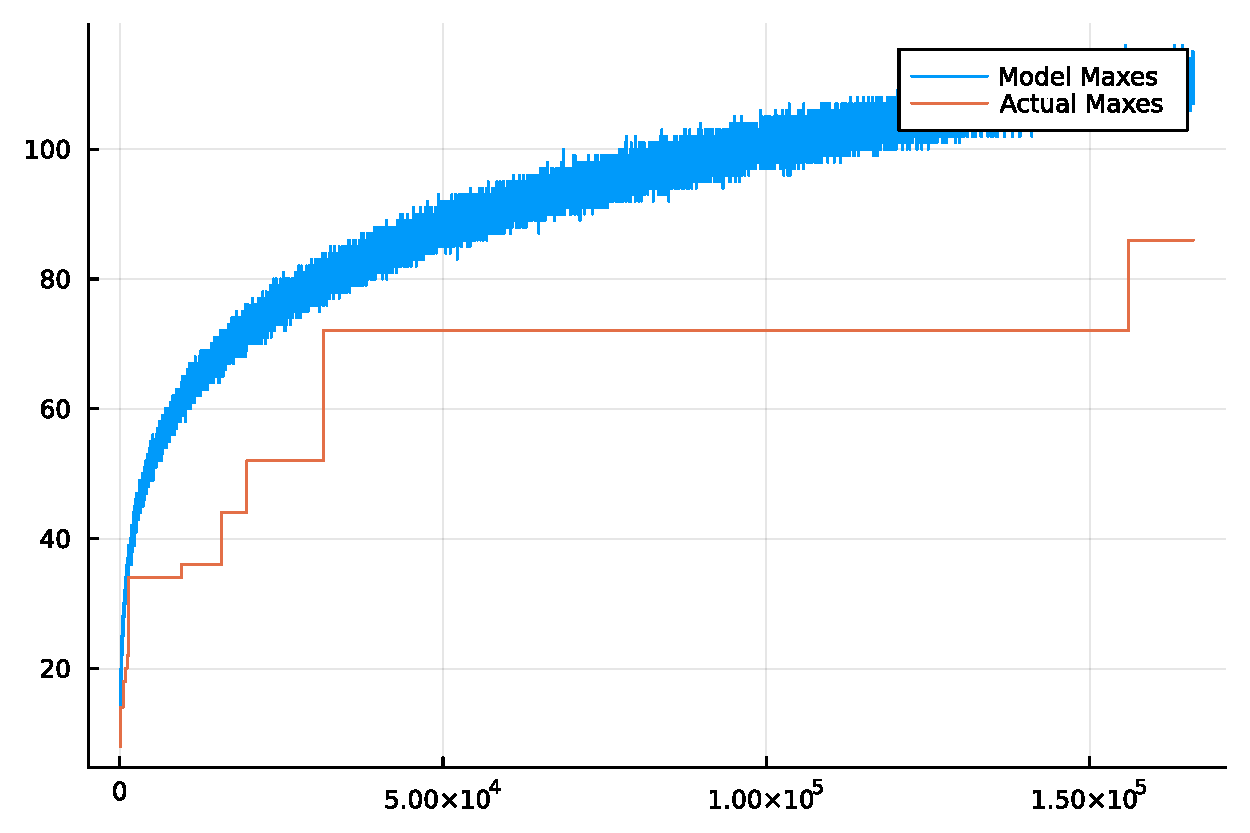
\includegraphics[width=\linewidth,keepaspectratio]{random-plot1.pdf}
  \caption{Maximum prime gaps, size of largest gap $\le n$ vs. $n$.}
\end{figure}

Well\ldots that's not quite exactly what we hoped it would be,
but it's also not all that bad! We can see that for rather
small values of $x$, the two graphs line up rather nicely,
and the two graphs approach each other again around $n = 30{,}000$
(it also seems that the 100 trials did its job fairly well in reducing
random variation). The two graphs do have their differences:
the actual prime gap graph is a little too jagged for our
(relatively) continuous-looking graph to model accurately. But it
still seems that they behave similarly in a way; one could imagine that
a curve of best fit through the actual graph would look rather similar
to our model. It's not out of the world either to believe that the next
jump in the prime gap will once again approach that of
our model for larger $n$.

So not all hope is lost quite yet! We still have some more ideas.
One first observation is that in the previous iteration of the model,
we restricted our ``fake primes'' to being natural numbers. Of course,
it perhaps makes sense to do so as primes are natural numbers, but
why should we restrict ourselves in that way? What if we take $x \in \mathbb{R}$
instead of $x \in \mathbb{N}$? After all, differences, logarithms, and
division are all just as well-defined on $\mathbb{R}$, so there's theoretically
nothing preventing us from doing this.

Obviously, when we deal with $x \in \mathbb{R}$, we can
no longer assign discrete probabilities to each element,
as there's an infinite number of them! Instead, we need
to assign an actual density function like the $\delta(x)$
mentioned earlier. But $\delta(x)$ poses some problems:
for one, the integral
\[\lim_{n \to \infty} \int_2^n \delta(x)\, dx = \infty\]
doesn't converge (perhaps unsurprisingly, as there are
indeed an infinite number of primes), so we can't hope to
use it as a probability density without at least some
modifications first. But for now, we can try something
simpler.

As our first step into using a continuous model, we'll
use the simplest possible density function: the uniform
distribution. For a closed interval $[a, b]$, we can
define the following uniform density function
\[f(x) = \begin{cases}\frac{1}{b-a}, & a \le x \le b \\ 0, & \text{otherwise}.\end{cases}\]
Then, since the prime number theorem predicts roughly
$n/\ln(n)$ primes less than or equal to $n$, we can
randomly sample $n/\ln(n)$ numbers uniformly from the
interval $[2, n]$ to get an approximate distribution of
primes. So we repeat the previous experiment, with the
only change being the switch to this new method of
generating our ``fake primes.''

\begin{figure}[H]
  \centering
  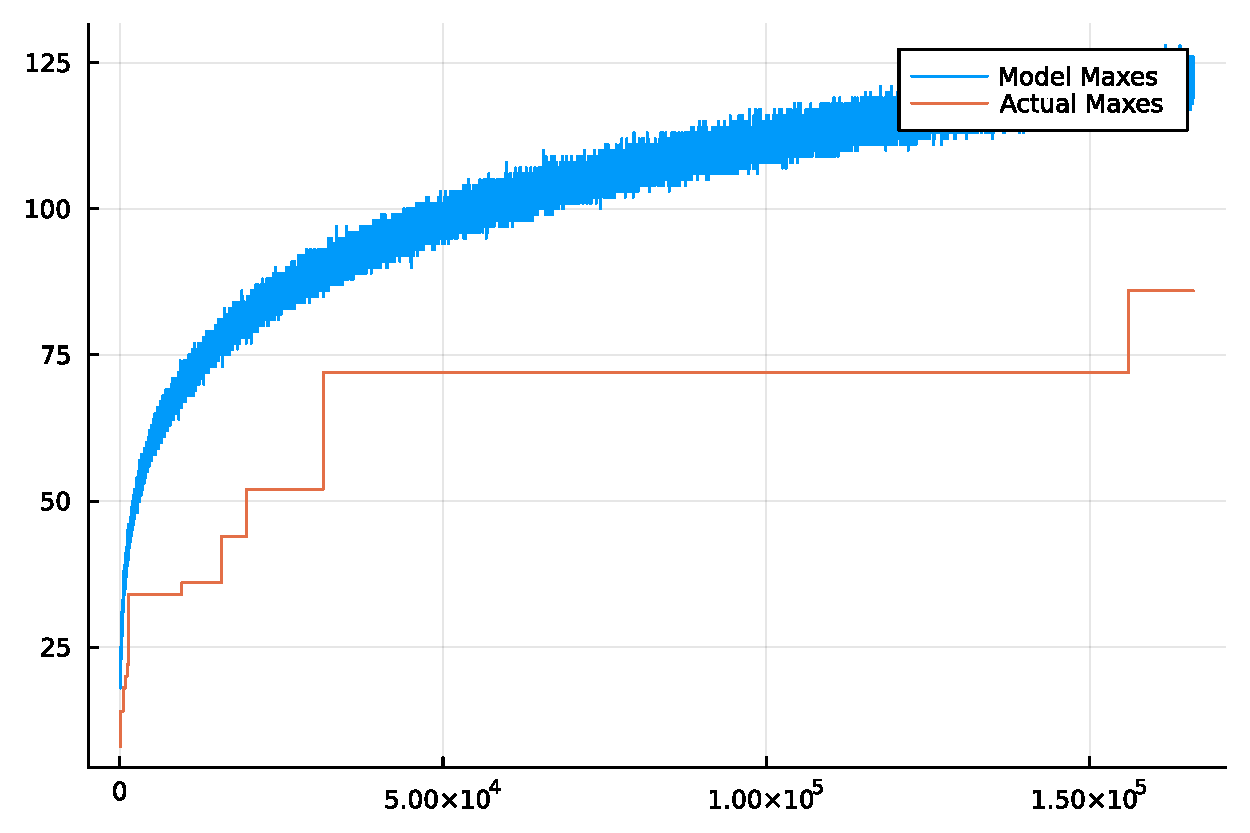
\includegraphics[width=\linewidth,keepaspectratio]{random-plot-with-reals.pdf}
  \caption{Maximum prime gaps, size of largest gap $\le n$ vs. $n$ (uniformly random).}
\end{figure}

Wow, that's even worse than what we had before, which is actually rather surprising.
We know that the prime number distribution is generally skewed to the right, meaning
primes occur less frequently for larger $n$. This would suggest larger gaps for the
than a uniform distribution would predict, but that's clearly not the case here. So,
what went wrong? We have to recall that the $n/\ln(n)$ value
from the prime number theorem is only an approximation. In fact, despite being
asymptotically correct, it actually has a rather larger margin of error. We
can immediately see this by plotting $\pi(n)$ and $n/\ln(n)$ on a graph.

\begin{figure}[H]
  \centering
  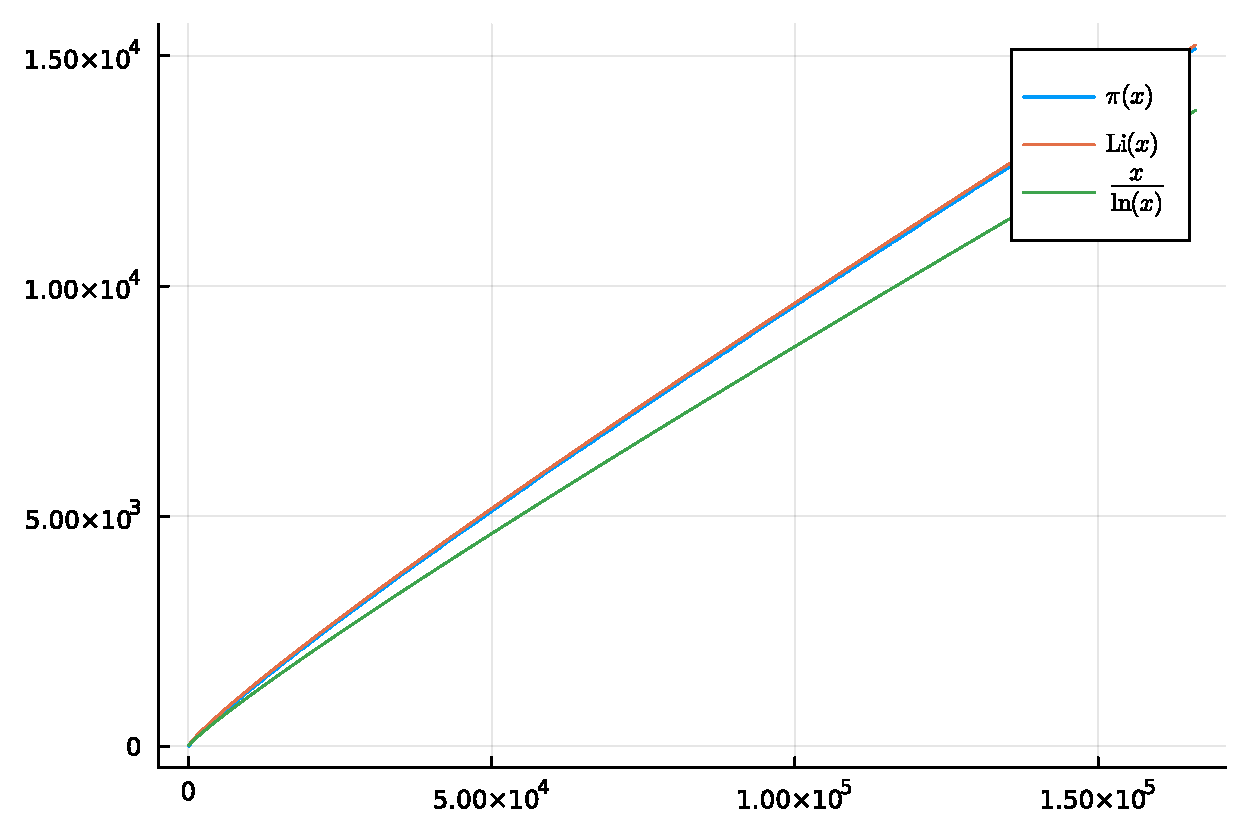
\includegraphics[width=\linewidth,keepaspectratio]{pmt_comparison.pdf}
  \caption{Number of primes $\le n$ vs. $n$.}
\end{figure}

We can now see that despite being asymptotically correct,
$x/\ln(x)$ is actually an underestimation to
$\pi(x)$, which explains the larger gaps our model
predicted. We also see that $\mathrm{Li}(x)$ is a much
better approximation to $\pi(x)$ than what the prime
number theorem gives directly, almost exactly overlapping
$\pi(x)$ from what we can see in the graph. Using
$\mathrm{Li}(x)$ instead as our metric for how many
numbers to sample, we recover most of the accuracy of our
first model.

\begin{figure}[H]
  \centering
  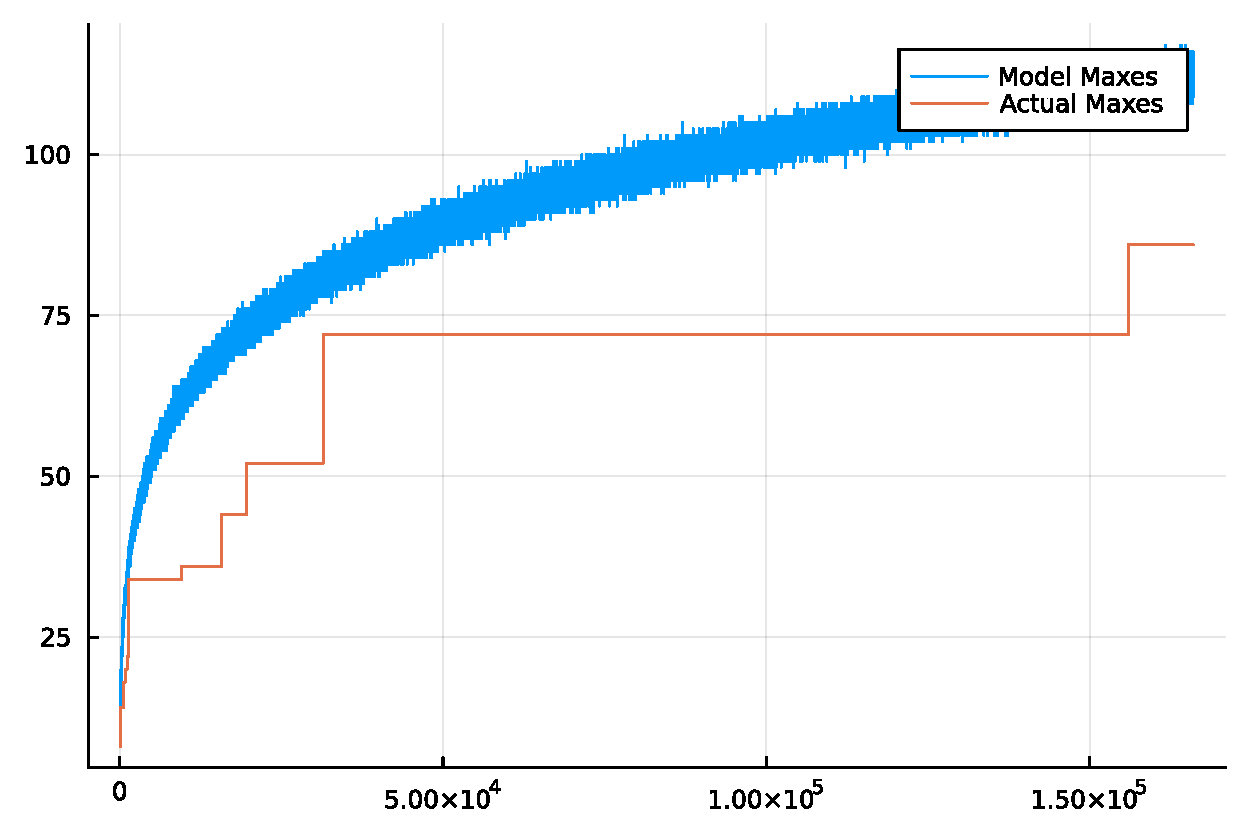
\includegraphics[width=\linewidth,keepaspectratio]{random_model_li.pdf}
  \caption{Maximum prime gaps, size of largest gap $\le n$ vs. $n$ (uniformly random using $\mathrm{Li}(n)$).}
\end{figure}

\section{Applications}
So, why might we care about a random model of the primes?
One motivation is that random models are generally much
easier to study than the actual primes themselves.
Mathematicians have a lot of probability and statistical
theory built up to analyze random variables, so as long
as we can achieve a good enough random approximation, we
can potentially analyze much more about how primes behave.

A second, perhaps much more tangible, reason is
computational efficiency. Finding large primes is
generally a rather difficult task. For example, the naive
trial division algorithm for finding primes requires
$O(\sqrt{n})$ time for every number (without even
accounting for the fact that basic operations like
we take for granted as $O(1)$ like multiplication also
start to slow down for very large integers),
so we can imagine that
using this method to find very large primes soon becomes
too inefficient. A much better method is to
use a sieve (the sieve of Erastosthenes, for example),
which finds many primes at once by removing multiples of
known primes. Sieve algorithms can bring time complexity
down to near $O(n)$, which is indeed already pretty good. 

But notice that this $n$ captures the value of the largest
integer we want to test. That means as soon as we want
to go from $n$ to $n + 1$, we have to run the entire
$O(n)$ algorithm all over again just to test that one
extra integer. This is where the power of the random
model comes in. Assuming that random number generation
is $O(1)$ (we'll assume this mainly for simplicity),
the random model algorithm is $O(k \log(k))$ (the
$\log(k)$ factor comes from sorting the random numbers,
which could be an area for improvement) in the
width the interval $k$. The random model will be much
more efficient for intervals containing very large
numbers but of reasonable width, as it doesn't need to
waste time in the smaller numbers to sieve out primes
correctly. This constraint is arguably pretty reasonable,
as we tend to perform experiments in iterations anyway.
That is, we can check the intervals $[n, 2n]$, $[2n, 3n]$,
and then $[3n, 4n]$ separately without having to worry
about duplicating work. But there's something even better.

A big problem with randomness is that, well, it's random.
Random data tends to contain a lot of noise that we don't
want, and we typically try to reduce this effect as much
as we can by conducting many trials. This may seem like
a problem, as running many trials will surely slow the
model down and add a huge hidden constant to our
$O(k \log(k))$ time complexity. But there's an easy fix:
what about the trials requires that they need to be run
in sequence? The whole point is that we run independent
trials to reduce random error, so we can simply
run them \textit{in parallel}.

Even the weakest among modern computers these days have
several cores, so we can easily take advantage of
\textit{multithreading}. We can simply run as many trial
as we can in parallel, which will significantly reduce
the impact of running many trials. In the Julia
programming language, this is as simple as
prefixing a for loop with the built-in
\verb|@threads| macro. In our experience, running
multithreaded on only 4 threads yielded over a
two-times speedup, which is already very impressive
for such little modification to our original code.

\section{Extending Cramer's Model}

The fundamental idea of Cramer's model is quite powerful. For any seemingly random set of numbers, we can emulate its density by using a random distribution. An interesting point of extension is, can we use this idea for similar sets of numbers other than the primes?

We introduce a lesser known sequence of numbers known as the Ulam numbers, named after Stanislaw Ulam, who first popularized the sequence in 1964. Let $U_n$ denote the n-th Ulam number. The sequence starts with $U_1 = 1$, $U_2 = 2$. Then for $n > 2$, $U_n$ is the smallest integer greater than $U_{n - 1}$ that can be written as a unique sum of two distinct earlier terms. The first twenty Ulam numbers are:
\begin{gather*}
  1, 2, 3, 4, 6, 8, 11, 13, 16, 18, \\
  26, 28, 36, 38, 47, 48, 53, 57, 62, 69.
\end{gather*}

% Psuedorandom similarity to the primes
Similar to the prime numbers, the Ulam numbers are a deterministic set found by a clear procedure. Once again, there are no equations to describe where Ulam numbers will show up on the integer number line. Let's run a program to see the distribution of Ulam numbers across a larger sample. Finding Ulam numbers effiently is a difficult task in itself, but we can do it naively. 

\begin{figure}[H]
  \centering
  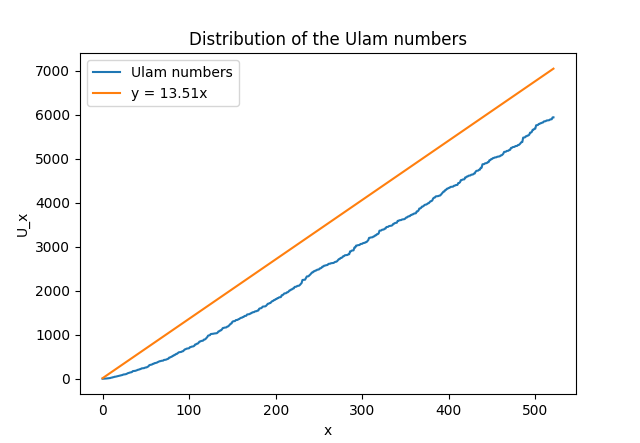
\includegraphics[width=\linewidth,keepaspectratio]{../images/Figure_3.png}
  \caption{Distribution of the first few hundred Ulam numbers}
\end{figure}

As can be seen by the distribution, Ulam numbers look quite linear. It has been shown that the first 3 million terms are close to the line $y = 13.51x$ \cite{b2}. Interestingly, Ulam himself conjectured that the natural density of Ulam numbers is 0. This means Ulam believed the distribution of Ulam numbers eventually converges to 0. But, as it turns out, calculations up to around a billion indicate that this is probably not the case. The observed density actually converges to around 0.074 \cite{b2}. 

% Revise this:
Using this density and the fact that Ulam numbers look to be quite linear, let's try to apply Cramer's model. For each natural number $x \ge 1$, we define the independent probability that it is an ``fake" Ulam number to be \[p(x) = 0.074\]

An example run of this model gives us something that looks very similar to the line mentioned earlier.

\begin{figure}[H]
  \centering
  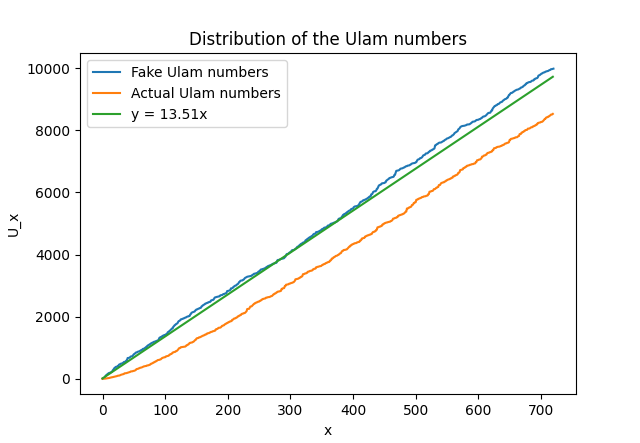
\includegraphics[width=\linewidth,keepaspectratio]{../images/fake_ulam.png}
  \caption{Distribution of random model vs the actual Ulam numbers}
\end{figure}

The Ulam numbers appears to be well below our estimated model. But, that is largely due to our relatively small range of $x$. As we look further down the Ulam sequence, the density 0.074 will become a better approximation.

Throughout this paper, one natural question that may arise is: why do we care about a heuristic such as Cramer's model? To answer that question, let's consider an analag to the Twin Prime Conjecture, but for Ulam numbers. The Twin Prime Conjecture states that there are an infinite number of prime pairs of the form ($p$, $p + 2$) \cite{b3}. Bringing over this idea to the Ulam sequence, we might speculate that there exists an infinite number of Ulam number pairs $(x, x + 2)$ in the Ulam sequence. (Because Ulam numbers can be odd or even, we could change the conjecture to consider pairs $(x, x + 1)$. However, this is not backed heuristically, as there have only been 4 such pairs in the first billion Ulam numbers \cite{b2}. So, we will go with the slightly looser conjecture). 

Proving this conjecture for the Ulam numbers does not have any clear consequences. But the point in this exercise is to show the power, and perhaps the flaws, of Cramer's random modeling technique for these types of sequence. So under the assumption that our random model accurately models the distribution of Ulam numbers, we will show that our conjecture is true.

\medskip\noindent
\textbf{Proposition.} \textit{Under the assumption of accuracy of Cramer's model for Ulam numbers, there exists an infinite number of Ulam pairs of the form ($x, x + 2$)} 

\smallskip\noindent
\textit{Proof.} Let $U$ denote the set of Ulam numbers. According to our model, the independent probability of a natural number being a Ulam number is
    \[p(x) = 0.074\]
Thus, the probability that natural numbers $x$ and $x + 2$ are both Ulam numbers is
    \[P(x \in U) \cdot P(x + 2 \in U) = 0.074^2\]
Then the average number of ``Ulam pairs'' below some integer $n$ is
\[\sum_{x = 2}^{n}0.074^2\]
From here, it is easy to see that
\[\lim_{n\rightarrow \infty} \sum_{x = 2}^{n}(0.074)^2 = \infty\]
Thus, there exists an infinite number of Ulam pairs.
\hfill$\square$\medskip

As you can see, this proof is very simple. Using the idea of Cramer's random model, we can give very quick answers to conjectures like our analagous Twin Prime Conjecture. In fact, going back to prime numbers, an assumption of a modified version of Cramer's model being true can be used to give affirmative answers to all four of Landau's problems \cite{b1} (which includes the Goldbach conjecture, Twin Prime conjecture, Legendre's conjecture, and the question of near-square primes).
% https://chance.dartmouth.edu/chance_news/for_chance_news/Riemann/cramer.pdf

The key assumption in all cases is the accuracy of the model. Our assumption that the density of Ulam numbers converges to the constant 0.074 is only statistically shown, not rigorously proven like the prime number theorem. But, the main idea still stands. With any sequence of significant natural density, Cramer's model gives us a way to confidently guess its asymptotic statistics. Proving these results rigorously is far more difficult, but by random modeling, we can get the next best thing, which is a statistics backed guess. 

\section{Improvements to Cramer's Model}

Although Cramer's original model makes a fair attempt at estimating prime number distributions, it is flawed. Cramer's model can be thought of as a sequence of random variables, all with the independent probabilty $1 / \ln(n)$. This assumption of independence is what mainly makes proving long unsolved conjectures relatively trivial. But just thinking intuitively, independence between every one if these variables makes no sense. For example, if some number $x$ is chosen to be part of our random model, shouldn't we reduce the probability that $2x$, $3x$, $4x$,$\dots$ are part of the model to 0? If we made this adjustment for our model, wouldn't it make it more accurate? However, then the question arises, where do we then ``redirect'' those probabilites? Its true that trying to make all such considerations just returns us to the original complexity of the primes. We don't want that, of course. But we do want to improve the model's accuracy, while still maintaining its main assumptions. Let's look at some ideas for improvements. 

% Should probably revise this section with more accurate improvements,
% http://projecteuclid.org/euclid.facm/1229619660
For any prime $p$, where $p > 2$, $p + 1$ is even and therefore cannot be prime. Currently in our model we do not consider parity, resulting in an arbitrary number of neighboring integer pairs. In fact with the original Cramer model, one can make a similar probabilistic argument to the one we made with Ulam sequence, to show that there exists an infinite number of prime pairs of the form $(p, p + 1)$. This is of course, a very bad prediction. Thus, how can we try to make Cramer's model more precise here. We can't just set the probability of every even number to 0 without other adjustments. This would essentially half the density backed by the Prime Number Theorem. One idea is to ``move" the probability of an even number $e$ being selected, to $e + 1$. So for each odd number (except for 3), its updated probability would be $1 / \ln(n - 1) + 1 / \ln(n) \approx 2 / \ln(n)$.
% Finish this section, extend this idea to numbers not just 2 coprime
% Model takes in another parameter w, which satisfies this

% Maybe talk about prime triplets?
% https://math.stackexchange.com/questions/1653536/show-that-we-cannot-have-a-prime-triplet-of-the-form-p-p-2-p-4-for 

(Add models highlighting differences?)
Cram\'er's random model uses this idea as a naive approach to emulate the distribution of prime numbers. Consider a random subset of the natural numbers, where the independent probability that a number $n$ is chosen is $1 / \ln(n)$. Let's call this random set $P'$, where $P$ is the set of actual prime numbers. Cram\'er conjectured that $P'$, which consists of our ``fake primes," accurately models the distribution of P. 

% Perhaps add summary of proof for this result
According to this heuristic, we have the resulting claim, which is known as Cram\'er's conjecture:
\[\limsup_{n \to \infty} \frac{p_{n + 1} - p_n}{(\ln p_n)^2} = 1\]
where $p_n$ denotes the $n$-th prime.

(Additional sections for these ideas (TBD)):
\begin{itemize}
  \item Problems with Cram\'er's naive model and ways we can improve it (with modern results)
  \item How Cram\'er's model fares depending on the size and location of the interval, calculating asymptomatic statistics
\end{itemize}

\section{Primality Tests}
One of the fundamental problems in math and cryptography is determining whether a large number is composite or prime. Since it is computationally difficult to manually calculate a sieve every time, there are many heuristics and methods to do it faster. A primality test is one of these heuristics/methods.

To start with, there's the Sieve of Erastothenes, which we encountered in the course. This is a fairly brute-force way of determining primality. A smarter way is through the \textbf{Fermat primality test}.

We studied Carmichael numbers in 2051. To redefine them, a Carmichael number is any composite number that satisfies the property, $\forall a \in \mathbb{N}$
\[
    a^{n -1} \equiv 1 \mod n 
\]
Carmichael numbers are significant since they constitute one of the significant shortcomings of the Fermat primality test. The Fermat primality tests is one of the more primitive methods of this still. Of course, it is still used and in some cases, are run before more advanced algorithms like Miller-Rabin or Baillie PSW.

With this in mind, there are two different approaches here, we can try to find all the Carmichael numbers or we could generate more efficient primality tests. In this case, the primality tests are more efficient because probabilistically, they are likely to give better answers. One of the common ways to do this is with the \textbf{strong probable prime test}. The test takes in two numbers: A number $n$, the number we are checking for primality, and another number a, $2 < a < n - 1$ which is coprime to $n$. Additionally, let's rewrite $n - 1 = 2^s d$, where $s > 0$ and $d$ is an odd integer. A strong probable prime in base $a$ is defined as a number $n$ that satisfies 
\[
    a^d \equiv 1 \mod n
\]
\[
    a^{2^r d} \equiv -1 \mod n, 0 \leq r < s 
\]
Why does this work? Well, firstly, if n is an odd prime, then it passes because of Fermat's little theorem, or Fermat's primality test. $n$ passes in this case because $d = n - 1$. In fact, Fermat's primality test alone defines a weaker notion of a \textbf{probable prime}. A probable prime is any condition that is satisfied by most primes. \\
The other reason this works is because the only of roots of $1$ $\mod n$ are $1$ and $-1$. A simple proof of this:
\[
    (x^2 - 1) \equiv 0 \mod n
\]
\[
    (x + 1)(x - 1) \equiv 0 \mod n
\]
\[
    x = 1\,\,\, \text{or} -1 \mod n
\]
With this, we now have the tools to construct the \textbf{Miller-Rabin test}. The variable a tells us if the number in question is composite or not. Of course, there are still composite numbers that can fool the Miller-Rabin test. However, there isn't a set family of numbers for this and it changes depending on the value of a and n. If a tells us that n is a composite, we call it a witness. If it misinforms us, we call it a liar. If we pass all the tests for Miller-Rabin, we classify $n$ as a strongly probable prime. It has been proven that the number of liars is at most a \href{https://doi.org/10.1016%2F0022-314X%2880%2990084-0}{$1/4$} of the values of $a$. In reality the number of liars is of course much lower for many numbers but we use this number to model the worst case. That means, depending on the number of times we run Miller-Rabin, let's say $k$ times, our probability of n being composite is $0.25^k$. To give an example of what this means, if we were using the fermat primality test, we would have little idea of how accurate our results were and would most likely be more computationally expensive to run to get similarly accurate results.

This is pretty great! At the same time, this isn't that good of a way to \textbf{generate} primes. While the Miller-Rabin test is good at determining primes, sieves are still the best way of generating them. In fact, if you compare them, the sieve of Erastothenes, the most basic sieve significantly outperforms the Miller-Rabin in time. However, we're not quite done with Miller-Rabin yet. While Miller-Rabin can never be quite as good as a Sieve, we can still optimize it. The only part of Miller-Rabin that is not deterministic are the randomizations. We can make this deterministic. Through some \href{https://doi.org/10.1145%2F800116.803773}{Group Theory}, we know that we only need to iterate till the minimum of $n - 1$ and $2\ln{n}^2$ since if we assume the Generalized Riemann Hypothesis, we know that every group is generated by the smallest $\ln{n}^2$. However, in practice, this is usually much more expensive and the normal Miller-Rabin is used since it has extremely high confidence.
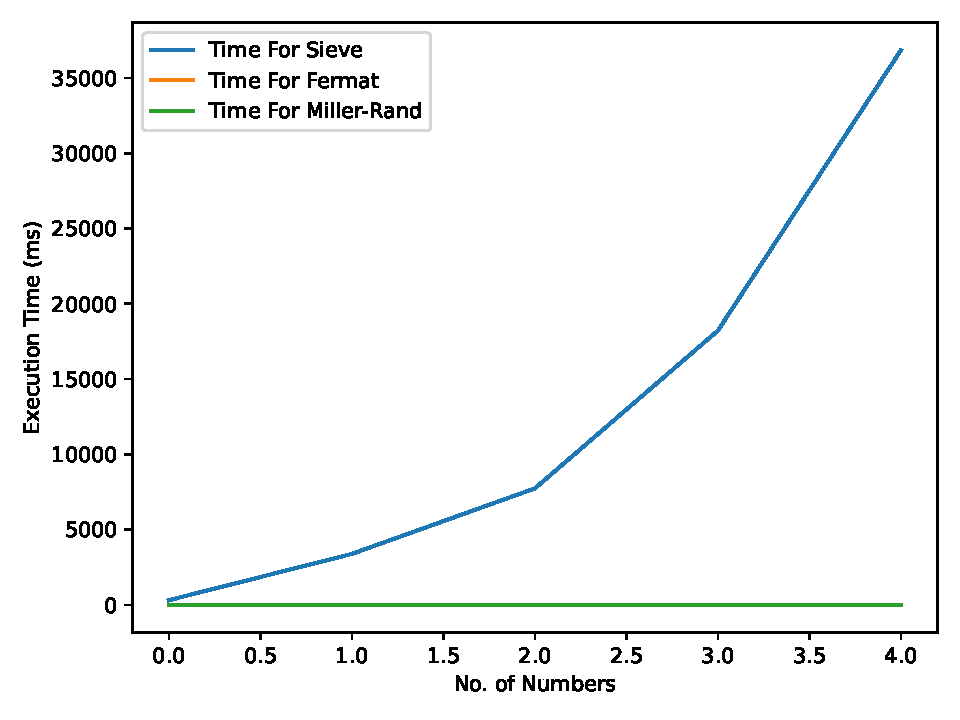
\includegraphics[scale = 0.31]{Fermat-Sieve-MillerRand.pdf}
With this graphic, you can see that in general, the Sieve is the worst way of finding whether a number is Prime, however, for certain numbers, the Fermat test can take extremely long, especially so for primes.
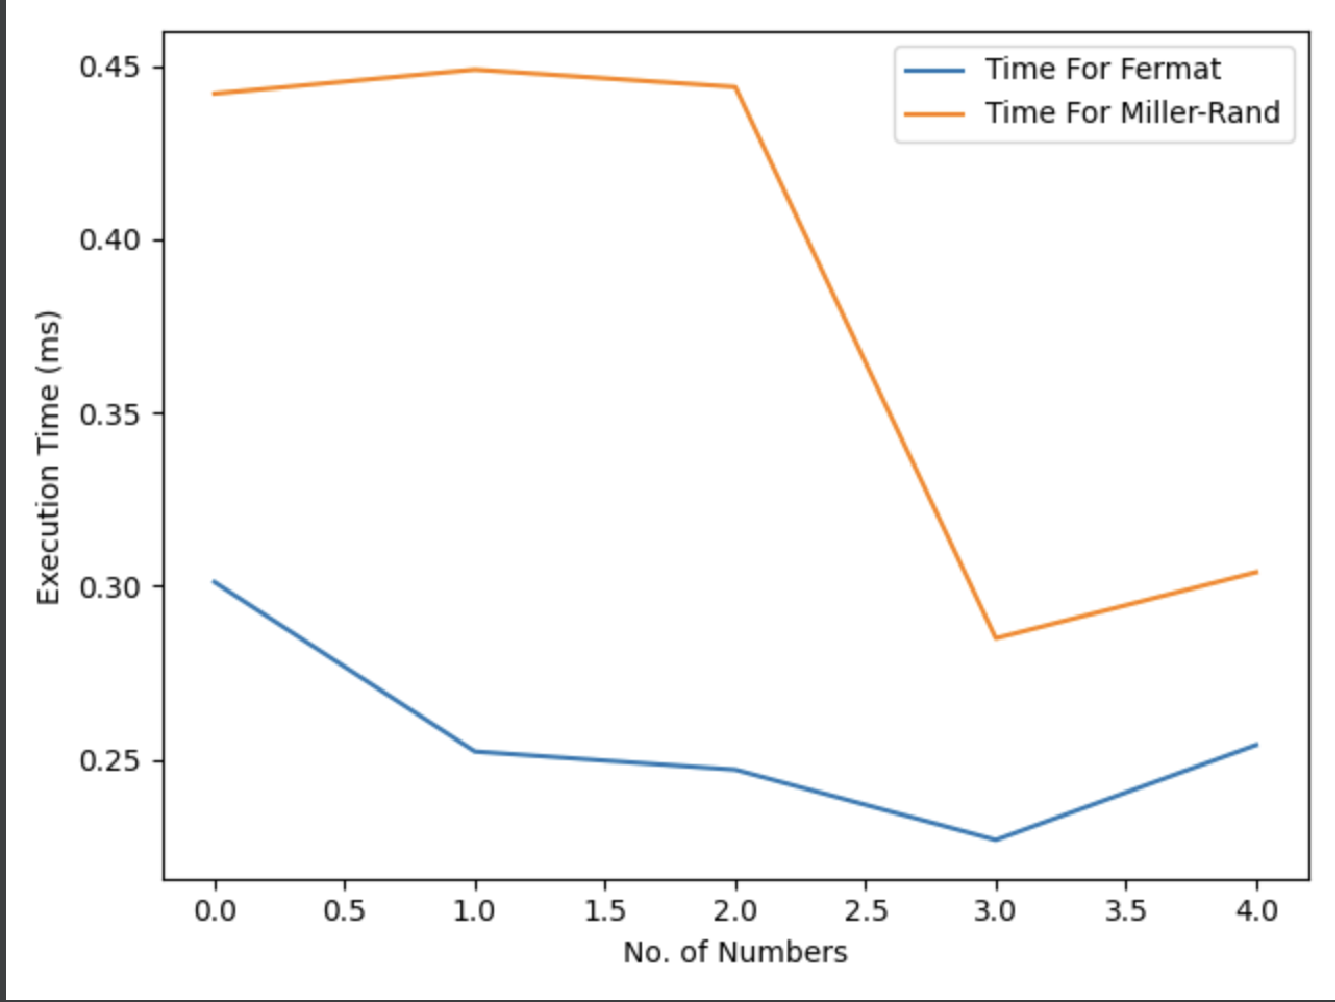
\includegraphics[scale=0.31]{Fermat-MillerRand.pdf}
In this graph, you can see that for the most part, they take similar amounts of time with the Fermat test taking less time since it's a weaker check.
% \[

% \]
\section{Extension/application/generalisation}
% You should change this section's name to something relevant to
% your project (e.g. "Applications of the RSA encryption
% algorithm" or "Linear Diophantine equations in $n$ unknowns"
\begin{itemize}
    \item Connections from Cram\'er's conjecture to the Riemann hypothesis
    \item Other ways to use Cram\'er's technique of random modeling
\end{itemize}


\section{Preliminary Code and Illustrations}
% Here should be some illustration of the concepts described above. Also place any code you used to generate the code (use the lstlisting package if this applies to you).

Cram\'er's random model allows us to heuristically test properties of primes.
In this example, we graphically compare the maximal prime gap of the model and the actual primes.
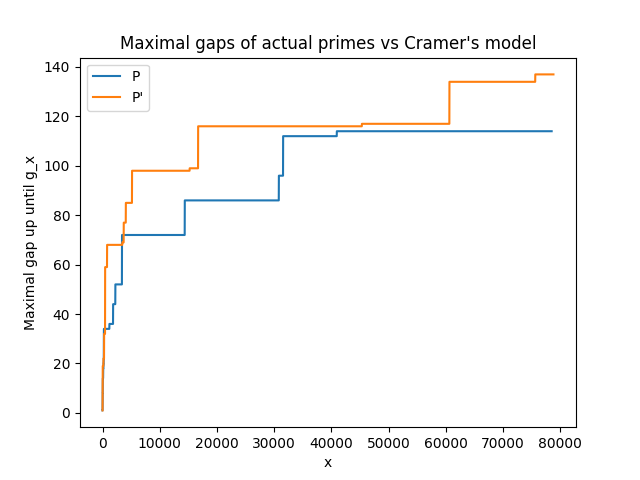
\includegraphics[scale=0.5]{graph.png}
% \inputpython{../models/original_model.py}{6}{37}

\section{Accuracy of the Model}
% You should change this section's name to something relevant to
% your project. This section allows you to reflect or conclude
% the work you have done in your project and discuss future work
% that could be done on the project (e.g. applications you tried
% to make but couldn't find the time).

Under heuristic testing with variations of Cram\'er's model, we should be able to support strong statements such as Bertrand's postulate and Legendre's conjecture. However, comparing with the actual primes, it should be clear that Cram\'er's model is inaccurate. Further work would involve the creation and tuning of other random models, to more closely emulate prime distribution.


\begin{thebibliography}{00}
    \bibitem{b1} \href{https://terrytao.wordpress.com/2015/01/04/254a-supplement-4-probabilistic-models-and-heuristics-for-the-primes-optional.}{Terence Tao, 254A, Supplement 4: Probabilistic models and heuristics for the primes (optional).}
    \bibitem{b2} \href{https://oeis.org/A002858}{OEIS Foundation Inc. (2023), The Ulam numbers, Entry A002858 in The On-Line Encyclopedia of Integer Sequences}
    \bibitem{b3} \href{https://arxiv.org/abs/1910.14674}{James Maynard, On the Twin Prime Conjecture}
    \bibitem{b4} \href{https://chance.dartmouth.edu/chance_news/for_chance_news/Riemann/cramer.pdf}{Andrew Granville, Harold Cramer and the Distribution of Prime Numbers}
% \bibitem{b3} Wikipedia Article on Prime Gap
% https://en.wikipedia.org/wiki/Prime_gap
\end{thebibliography}
\vspace{12pt}

\end{document}
